\documentclass[oneside]{book}
\title{The Maiden Who Travels The Planet}
\author{Author: BennyMatsuyama\\Translation: XComp\\Typesetting: \def\swindlesmccoop{swindlesmccoop.xyz}}
\date{December 15th, 2011}
\usepackage{graphicx}
\usepackage{graphics}
\usepackage[margin=100pt]{geometry}
\usepackage{indentfirst}
\usepackage[T1]{fontenc}

\usepackage{fancyhdr}
\fancypagestyle{plain}{
    \lhead{}
    \fancyhead[R]{\thepage}
    \fancyhead[L]{}
    \renewcommand{\headrulewidth}{0pt}
    \fancyfoot{}
}

\begin{document}
\maketitle
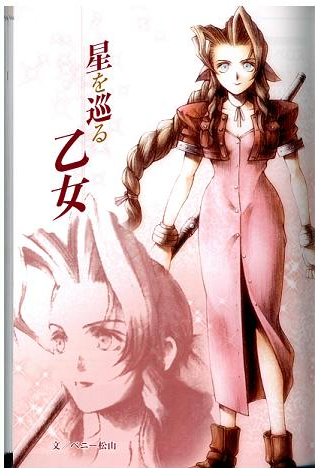
\includegraphics[width=\textwidth,height=\textheight,keepaspectratio]{cover.png}

\chaptermark{}
Underwater... Aerith was sinking. Lying stretched out with an expression as if she was asleep, she quietly sank into the cold and tranquil lake. The net of light scattered by the ripples of the surface danced upon her motionless body. It was as if it was trying to tie onto her.

Her kind face could no longer have those expressions that were full of energy. The feelings of joy and fun that would spread to everyone around her, the anger she had toward those who disregarded the weak, and the endless tears she had in sorrow... None of them were going to appear again.

Her body was going to be silenced for eternity.

However, that didn't mean the end of Aerith. She was watching. She wasn't watching through her beautiful green eyes, but through her soul... She watched within a discarnate body filled with the energy of life, as it overlapped her physical body. She watched as the surface of the lake drew further away. She watched as the human shapes gazed at her from the hazy other world. The world where things were alive was another world to her. She watched Cloud's face which looked as if his heart was going to fall apart from the sadness of loosing her, the anger and hate he had for her being taken from him.

“Don't blame yourself. There's nothing to worry about anymore. It's going to be all right even if Meteor falls. So don't let yourself be dragged down by those feelings. Just think about how you can be yourself.”

She tried to say it but her lips wouldn't move. There was no magic that would let her thoughts reach Cloud from her spiritual body as he disappeared fast into the distance. The light that twinkled on the lake's surface became weak and distant as she sank. She fell smoothly into the depths of the Cetra ruins, The Forgotten City. Aerith, the last remaining survivor of the Cetra had fulfilled her mission to protect the Planet. The final place where she was supposed to reach had no boundaries no matter where she went...

\newpage
Yes. No matter where she went.

She had reached the bottom of the lake. But even now Aerith continued to sink.

Her physical body was caught by a blanket of dust, like fine powdered snow, which had accumulated over immeasurable time, and was being engulfed deep into the bottom of the lake. It told of how she was now separated from her short twenty-two years of life for eternity. The vessel that had been separated from the soul was going to return slowly to the Great Earth in the pure water.

Aerith's consciousness was moving to the next, lower level.

Nothing changed as she breathed lightly in the dust that floated around her. Aerith continued to sink through the heavy layer of precipitation. The only thing she could see was darkness... But it was a warm, tender lightless world where she didn't feel lonely.

She soon realized that it wasn't dust or mud that she was feeling. Her senses had adjusted so that she could feel the things around her. Her five senses were at a higher level that let her feel the true nature of the objects.

The world she could see now was not of darkness.

She was inside some faint green light that wrapped around her. At the same time, she recognised what she saw. Energy that was split into thousands no, millions of streams were flowing and circulating around every nook of the Planet. The flood of light that engulfed her was one of the streams that separated from the rest. The amount of Mako energy that the Planet had was far beyond human expectation and could not be presented by mere figures.

Aerith watched as if the Planet was beating with life. She watched the brilliance of the Lifestream that drifted around. She recognized the source of life of which everything returns to.

It was a place full of energy where countless souls were merged together along with their knowledge and experiences. Even their memories were unbound from them. But Aerith was “whole”. She remained herself in the place where the consciousness of the dead flowed and swirled about, keeping the character she had when she was alive. She retained the consciousness of the Aerith Gainsborough she once was and she was now drifting with the Lifestream.

She didn't know that she would become this way.

As the last surviving Cetra, she had the role of maintaining the Great Earth's richness during her life's journey. Aerith talked to the Planet. She talked to the consciousness that was part of the Lifestream, that is. She was told that death was not the demise of life.

Most humans thought death meant that they would become nothing. Having their consciousness engulfed by darkness, never waking again, a nothingness that can't be comprehended, they thought death meant to be totally annihilated. That's why humans feared death. They were afraid of losing their existence. Even if they themselves realized that they were a race that had a short lifespan, there were many that wanted to avoid it. Even those that had reached an old age after a fulfilling life.

Aerith knew that death didn't mean to be annihilated. She even knew about the world that a Cetra would reach in the end once they had fulfilled the mission they had on the Planet. That was why she accepted death fearlessly, even when she had a strong feeling it was going to happen to her some day soon. She fulfilled her mission as she meant to, without any fear. Her heart was at peace even though the humans, who had lost their power to speak with Planet long ago, said that she died an unnatural death. She had no regrets such as wishing she was still alive, or because she avoided her mission.

Even so, she was sad. Her heart was in pain.

All the companions that she had journeyed with, the people she grew close to for the first time, the mother that raised her and looked after her for fifteen years Elmyra, the people that she didn't know too well, the people who she might have met in the future, people she hadn't met yet... It was a fact that she could no longer be with the “living”.

Aerith also knew that the sadness was also with those who she left behind. They didn't know that she still existed as her soul. They didn't need to know. Even if she wished they did, the sadness wouldn't be healed if they knew the truth. The thought of everyone's sorrow made the pain in her even worse.

Aerith was in even greater pain when she thought about Cloud.

At first, she thought he somehow had some similarities to her first love. Even so, his looks, voice and personality weren't similar, and he also made her think of him as a mysterious person... But it soon didn't matter. She loved him much more than her first love. Cloud was her hero and he couldn't keep away from danger. She saw him as someone full of confidence, cool and gave the impression that he would disappear in an instant if she took her eyes off him. She wanted to stay by his side forever if she could. She really wanted to.

When she left her companions and headed for the Forgotten City, Cloud's heart was like an egg that was on the verge of cracking open. It wasn't going to crack open like the way an egg hatched, but as if only the yolk was going to seep out. It was as if his mind was going to shatter. She wanted to comfort him. If she wasn't the last survivor of the Cetra she probably would have done so without a doubt.

However...

The man in black and silver, who was once a hero, had taken over the will of the “Calamity that fell from the sky”, Jenova, and was in a state of madness. He was going to summon the most powerful destructive magic, Meteor using the Black Materia. Having been passed the mission from her Cetra ancestors, she had no choice but to carry it out. Sooner or later Sephiroth was going to summon the giant meteor that would surely inflict an enormous amount of damage to the Planet. It would cause a wound that could destroy the very Planet itself. Without doubt, the Planet would then concentrate a huge amount of the Lifestream to heal itself. It was Sephiroth's intention to make all that power his. After that, he would become one with the Planet and become something equal to a God. He would probably then burn all the humans he hates to death. The future of the Planet and the cycle of all life would all end as she knew it.

Aerith could sense from the whispers of the Planet that something could be done to prevent the worst from happening. She also knew that it was something that only she, the last remaining Cetra, could do. She could only obtain the indepth knowledge from the Forgotten City. But heading there also meant that she would become the greatest obstruction to Sephiroth's plans.

That was where Aerith hesitated. Would she let all humans die or was she going to avoid such a disaster in exchange for her life... But she never did think about it, and was already prepared. When she did hesitate about leaving Cloud in sorrow, she would think about how it wouldn't save her companions or the people of the world. She had already made up her mind. There was no other choice. It was all for Cloud too.

And so, alone, she set off for the altar that was in the Forgotten City to find out what she had to do. Indeed, the key was the last of the Cetra. It was the White Materia that was passed down by to her... As if it held the fate of the last remaining Cetra, this tool could summon the ultimate White Magic, Holy, needed to counter Meteor. It was the Materia that was entrusted to Aerith by her mother, Ifalna. She had never used it before and had always hidden it inside her ribbon, never leaving her. Finding out that she had it on her, she prayed with all her heart. Through the Materia, she talked to the Planet trying to summon the White Magic Holy that could destroy Meteor.

Even the slightest hesitance may have meant that her prayers wouldn't reach the Planet. But she did it. The requirements were fulfilled before Sephiroth struck her, after realizing her intentions. She accepted the death that she had felt long ago as the sword pierced through her.

She looked at peace.

But a cry came through to her.

It wasn't the sound of her cry. If it was then she would have felt the blood gushing up through her throat and the fury that forced its way out from the depths of her soul – It was the sound of Cloud's heart breaking. It was the cry of his heart that could never be healed of the grief he had towards Aerith's death, the blame towards himself and the hatred he had for Sephiroth.

She was surprised at the great sorrow he had for her. She was a little happy that he thought so much of her, but she also felt the pain that was many times greater. There was nothing she could do about Cloud's suffering, and the pain ached in her heart.

The pain continued even though she was in the Lifestream.

Although she had lost her body, she recognized the pain by creating an image of herself in her mind. Aerith looked down as she put her hands to her throbbing heart... Before long, she realized something.

All around her was the existence of countless numbers of consciousnesses. There were lots of voices and an abundance of memories. Everything around her was something that she never felt when she was in the church in Midgar. Like her, the souls of those that had died had returned to the Planet and were all here.

Even so, she couldn't see anyone nearby that had a form like she did. From what she saw, only she retained the image of her past self in the mist of the flowing energy full of different consciousnesses.

“I wonder... Is it because I'm a Cetra?”

The words came out as a murmur from Aerith. Here, words and thoughts were the same. As an entity of consciousness, her thoughts and feelings were only expressed as waves she emitted. Similarly, the huge number of memories in the Lifestream also reached her as all sorts of waves. All around her she heard whispers of how if you didn't retain a strong ego, you would soon no longer know which consciousness belonged to you.

“I was hoping my words would reach Cloud...”

She puffed out her cheeks a little looking displeased. She was not affected by the confusion of the various consciousnesses that existed in the sea of memories and knowledge inside the Mako energy. Because of her experience of hearing the voice of the Planet when she was young, she had built up a lot of patience. Aerith was raised so that she could retain her own consciousness and not lose her personality.

But she understood returning to the Planet depended on how she was separated as a whole. Even when water droplets fall into a river, they blend in and can't be seen anymore. No matter how used to things she was, she thought it was odd how her soul could still remain unique in the vast sea of conscious energy.

“If it's because I'm a Cetra, then the Lifestream should be full of Cetra. My mother died and she was also a Cetra... But it's been fifteen years. Maybe I'll become one with the planet and slowly disappear?”

Slanting her head to the side, she thought more about it.

“Will I be able to talk to Cloud somewhere? So that I can tell him I'm fine... It's kind of odd saying I'm fine, but maybe I'm ‘still me' down here?”

Maybe she could be clear about her affections towards Cloud here. While living in Midgar, there were several times when she sensed souls that had died in faraway lands coming to Midgar to see their families or loved ones one more time— to tell them that they loved them. Those who still had those feelings, or had those feelings left behind them could strongly retain their consciousness as a whole.

“But does that mean I'll disappear as soon as I meet Cloud? I wonder if that's what's happening or... Is there still something else I've still to do...?”

At that instant, Aerith felt something like an electric shock surge through her. She clenched one of her hands into a fist and hit the palm of her other hand, as it struck her. It was only her imagining her phantom self hitting her hands together, but she could clearly hear the “clap”.

“It makes sense. There's a meaning to all this. There must be some reason why I haven't merged with the Lifestream yet. Like, how I was the only one in the world who had the materia to call Holy... There might still be something left that I have to do.”

Just when the thought crossed her mind, she felt a little commotion from the Planet. It wasn't from the individual consciousnesses but the Planet as a whole as if to confirm what she was thinking.

“...I see. I wonder what it is.”

Her question was answered with silence. The Planet too had yet to know what it was.

She smiled like the flowers that she used to sell in the slums. In the gentle fluorescent light, the smile that was loved by everyone bloomed sweetly.

“It's OK. There are still people I have to help. I can't rest yet. Until that time comes, I'll wander around here for a while. I'll spend my time here in the Planet... In our Promised Land...”

Wishing she could send away her thoughts, Aerith looked up at the sky... She looked beyond the shell of the Planet above her head. The particles of Mako that floated and shot around looked like the night sky to her.

She looked up into the sky like the time she sat beside Cloud around the kindling fire in Cosmo Canyon.

\newpage
In this world of Mako – Aerith knew that the concept of time and distance was different from the surface. Time seemed to flow by slowly, and if she wanted, could also flash by in the blink of an eye. The passing of time in the Mako held no meaning in the first place. The Planet's history was made up of accumulated memories, all merged together and were always by her side. There were memories of the present and also of the past. There was no way that Aerith could have seen all of them, but the events that were inscribed into the memories had surpassed time and were all linked together as a whole. It hinted that time was moving into the future in the world of the living. As those new memories from the surface merged together with the Planet, new life would be brought into the world as the energy from the Planet is delivered. That cycle told her how time flowed by one period after another.

Everything was linked to the insides of the Planet through the Lifestream. Even on the surface, in the most distant places, the flow of conscious energy would be delivered. On the other hand, there were places that were so close, but yet, the energy couldn't reach. There were areas that existed where even the winding flow of Mako can't get to. Aerith thought it must be the fault of all the Mako reactors. The energy was never meant to be used that way and if they continued to draw it out by force, it would eventually upset the balance. If the Planet could help humans live an easier life, then it probably would have done so. But Shinra Inc. was going too far. If their greed was to continue, then the equilibrium of the Planet's life would collapse... Aerith remembered how flowers would only bloom in the church and how the city of Midgar was drenched in Mako.

“And that's why the people of Shinra wanted to know where the Promised Land was. A land abundant in Mako energy, where only the Cetra knew how to get to... But that place is here. It's the place where everyone will go in the end, so they can return to the Planet. The land where Shinra could obtain all the energy they wanted didn't really exist, did it? It was all just a mistake.”

She murmured as she let herself drift with the Lifestream. She gazed at the moving Mako world that had very little change.

“The Promised Land that Sephiroth had in mind was much different. He was trying to create it all by force. He was going to wound the Planet on purpose so that almost all the energy would gather in one place. So that he himself could control it all alone. That was Sephiroth's Promised Land...”

Aerith shivered as she imagined what the Planet would be like if that happened.

“I wonder if Cloud and the others are all right... Tifa, and Barret. I hope they aren't pushing themselves too hard going after Sephiroth...”

“...Cloud? Tifa? Barret?”

The waves of one of the consciousnesses right beside her expanded as it reacted to her words. She rushed to leave the current she was in because it was the first time she came across another firm consciousness other than herself. When she reached the place where it came from, a shadow rose from the Mako. It wasn't as clear an image as Aerith but she knew it was the remnant of a female.

“You know them? Who are you?”

“I'm...”

It seemed her memory was muddled. It was probably because most of her soul had already merged with the Mako. But her core hadn't faded and was still drifting there as a whole.

“Oh, I have to introduce myself first. I'm Aerith. Could you be one of Avalanche's members?”

“Avalanche... Yes, yes that's right.”

The memories she had were being reconstructed from the Sea of Mako. Realizing who she was once again, her transparent figure rapidly returned to the form she had when she was on the surface. As if Aerith had some influence on her, the colours also came back to her.

Compared to Aerith, she still looked faint, but she looked human now and the clothing she had worn also reappeared. Her hair was tied back in a pony tail so that it wouldn't get in her way and her clothing looked like that of a soldier. She too had arrived here too early, she was about Aerith's age.

“How stupid of me to forget... I'm Jessie from Avalanche. Hey... Are you Miss Aerith?”

“You can just call me Aerith.”

“Thanks, Aerith. You know Cloud, Tifa and Barret, don't you? How is everyone? Are they still fighting Shinra? Oh...”

Jessie shook her head as if to apologize. “You must be like me now that you've come here.”

“Don't worry. I'm sure they're all fine.”

She changed her thoughts as she tried not to think about Cloud. Here, she couldn't lie so she had to not think about it.

“There was something that bothered Barret for a long time. So at that time you were... You were one of the people from AVALANCHE who were trying to protect the Sector Seven pillar. I only met Mr. Wedge...”

“Wedge?!”

Jessie's eyes widened. “Yes, Biggs too! All three of us arrived here together but lost sight of each other... Yes, until just a moment ago, I couldn't remember anything. Until I met you, Aerith.”

As if guided by Jessie's memories, two more figures appeared. The forms of a man with a thin beard and another that was stout bodied rapidly formed together.

“Wo- Woah.”

The bearded man, Biggs stared at the palms of his hands. “I'm still me. I thought I was going to disappear.”

“I'm so happy I can see the two of you again. And... You're the one that nursed me that time, Miss... Aerith? Did you die too?”

Instead of giving the obvious answer, Aerith nodded with a smile.

“It's been a long time, Mr. Wedge. It's nice to meet you, Mr. Biggs. After that, I became a member of Avalanche too so that kind of makes me a junior to all of you, doesn't it?”

“Hmmm, that kind of shows how dangerously high the death rate for Avalanche is, doesn't it?”

“Is Barret still the swagger of a guy he is? Well, he is quite a likeable guy.”

“Junior? I'm too happy! It's always been my aspirations to be a senior!”

After that, Aerith told all three of them what Avalanche was fighting for now. It wasn't just Shinra Inc. anymore but also with the much more dangerous existence known as Sephiroth... They had left Midgar to stop his evil ambitions of making the Planet his.

“So Cloud's become one of us now... I'm so happy.”

“Heheh... He's a cold guy but I knew he would join us.”

“Does that mean Mr. Cloud is a junior too? He's going to be tough to deal with.”

There was a lot of commotion among the phantoms of the Avalanche members as they laughed and smiled. But in the end, Aerith noticed their sadness. Some deep remorse bound the three of them together.

“What's wrong? All of you look like you're in pain...”

“Well... It's because of the way our lives ended. We can't redeem ourselves now.”

Jessie looked down sadly as Biggs continued.

“We fought with Avalanche because we had the same sympathy and thoughts. We thought that it couldn't be helped to have a few sacrifices if we were to stop Shinra. But we were completely wrong. We understood that when we came here... You know about it too don't you, Aerith? About the explosion of the First Sector Mako Reactor.”

“Yes... The First Sector was right at the other side of the slums I lived in. We weren't told much about it, but we heard quite a lot of people died...”

“At that time, we only thought that they were getting what they deserved if they got caught in the explosion, since they were all people that worked for Shinra on the upper plate. But in the end, all of us ended up here whether we worked for Shinra or not. So we fve been thinking about why we did it. All we were really doing was raising our voices and shouting out our opinions like drunks. We were just over-exaggerating about how we were saving the Planet...”

“...I didn't think about it that much either. I didn't want a minor role in life. I wanted to shine. So I thought by joining Avalanche, I could be a hero who could save the future of the Planet and that's all I thought about... I never imagined that it would get others involved. It's just so foolish...”

Wedge lowered his head in embarassment.

“The whole plan was actually drafted by the old Avalanche which no longer exists anymore.”

Jessie went on regretfully, “There were many more members in Avalanche and they were a much more extreme group. We only inherited the name of their resistance group, “Avalanche” from those people who are no longer around. But details of how to make a bomb and the plans of where to set it were left on a computer. Since I was good with machinery and bombs, I decided to try it... But I'm sure that plan was never intended to be used to just disable Mako Reactor One. The people that came up with the horrific plan hated the Shinra. They hated them so much that they would go as far as sacrificing lots of people... I should have realized it. Barret knew nothing about it.”

“That's why we...”

Dejected, Biggs looked up to the sky. “Why we wanted to merge with the Planet right away. We wanted to disappear. I remember now. But it was impossible. Barret's fighting to save even more people. We can't do any of that to atone for our sins. We can only be here and continue to suffer.”

“In the end, it was all too easy for us to forget who we were because we wanted to be at ease here.”

“It just didn't work. When we had the chance, we would revert to the way we were. Even then we're not as clear an entity as you are. It's kinda like a curse.”

They all laughed with self-derision until it all ended with a sigh.

“But... But.”

Aerith tried to comfort them with her words.

“Everyone's been wrong before. Even I've given people too little change when selling flowers before...”

“Hmmm... I really can't compare my stupidity to that.”

“But for all of you to have to keep suffering, it's just...”

“Thanks, Aerith. But as a senior in Avalanche, it's such a shameful story. All that big talk feels like it's backfired on me.”

“I really can't forgive myself. That's why this is the only way I can be here.”

“Someday, the day may come when we can return to the Planet but right now, we can't. Now go, Aerith. You must be in that form because there's a role you must fulfil. We're worried our sinful memories will transfer over to you.”

“No...”

“And then we'll suffer even more. So go, please?”

Jessie was lying. Aerith knew that she was trying to get far away from her so that she wouldn't have to share their pain.

The phantoms of the three people were fading. Aerith bit her bottom lip as tears welled up.

“Please let me say this at least. That day, many people managed to escape because the three of you worked hard to protect the Sector Seven pillar. I'm sure the number of people that managed to escape was more than the people who died in Sector One... And I also managed to save Marlene because of that. Maybe that isn't enough to free you all... I know that people's lives aren't something you add and subtract with but... Please remember that it's not only sins that you carry.”

“...Thank you. Thank you, Aerith.”

The voice of someone that no longer knew who they were echoed and they were taken back to the prison that they had decided for themselves. They sank into the sea of memories.

Aerith wiped away her tears and started walking again. She prayed that the souls of the Avalance members would be able to rest in peace soon.

\newpage
Aerith didn't know how much time had passed on the surface. Had it been days since she met Jessie and the others, or was it just moments ago?

She wondered if their pain could be healed by themselves. As she asked herself that question, she continued to travel the underground world. She drifted in the Lifestream in the Planet's Sea of Mako.

When she saw the next phantom, she held her breathe.

The point of a steel tube rose from a swirl of faint light. When she realized that it was an artificial hand linked to an arm, she thought that Barret too had left the world of the living. Aerith was sure that she had escaped Midgar with her mother Elmyra. Her heart tightened as she thought of Marlene.

“Marlene!”

Aerith's waves of thoughts expanded and they reached the phantom. The full figure of a man with a gun attached to his arm rose from the Mako. The weapon emitted a cold glow from it but it was from his left arm. The gun was fearsome as if it was physically real and the man's faint figure was stained in red.

“You're...”

“A woman... Where have I seen you before? You even know Marlene's name.”

“We've met haven't we, Mr. Dyne.”

He was Dyne, the governor of Corel Prison, an exile land full of sand and scrap. He was also once Barret's close friend. After what Shinra done to his hometown, his despair made him irrational and falling into a state of madness, he slaughtered many people.

“Ah, I see. You're the girl that was with Barret. Then that means you must be dead too. What a pity.”

Not believing what he saw, Dyne laughed. “I can't believe that after killing so many people, I would end up in the same place as an innocent girl like you after I die. This world truly is absurd. What a boring thing this Planet is. Everything really should be destroyed.”

“Is that what you still say?”

Aerith's figure stood in contrast to Dyne's. She raised her slender eyebrows.

“Even though you really care about Marlene?”

“Who cares. Girl, you-”

“I'm Aerith.”

“Heheh... You're a strong one. My left arm is all that remains of my past life. Fine. I'll call you by that name. You heard what I said that time, didn't you? The words I had with Barret. When I was trying to destroy everything, I was going to take Marlene with me here too.”

“You're lying. You were just bluffing.”

“I can't lie here, right? I was seriously thinking about it at that time to say the least. Then I challenged Barret to a deathmatch and became enlightened.”

For a while, Dyne laughed out loudly because of how he had to pay it all back with his right arm and his body. “And I thank Barret for that. After all, I've been swallowed up by the very “world” I wanted to destroy. I didn't want to end my own life. So instead, I wasted all those useless people that were scared in the exile land to free them and make them happy.”

“....”

“Do you see now, Aerith? Before you is the helpless, broken apparition of a man that even the Planet won't accept. The Planet that my wife Eleanor has already returned to. And I've already entrusted Marlene to Barret. Whatever happens to the Planet afterwards has nothing to do with me.”

“....”

Looking at how silent Aerith had become, he laughed again at how he managed to make the cheeky little girl back down. Then he realized that it wasn't funny and noticed that Aerith never took her eyes off him. He realized he didn't manage to make her back down at all. There was a glow in the gaze of her jade green eyes that made the madness in him back down.

“...You have no guts.”

“What did you say?”

“I'll say it again. You have no guts. You don't have the courage to go back and start over. You've only been tumbling round and round where it's the easiest going for you.”

As Aerith stared at Dyne, she took a step forward. Under the pressure of her powerful eyes, he hid his face with his gun and unconsciously stepped back.

“Barret also exchanged one of his arms for a gun. He said he would destroy the Shinra with his feelings of regret and hatred. That's why he too had his hands stained with the blood of many people. But he didn't fall apart. Besides taking on the burden, he's really trying to save the Planet this time. He's trying to protect the world that Marlene will live in without running away.”

“...Being able to change like that is that simpleton's strength.”

“Is Barret special and you're different?”

Dyne moaned at her question. He was waking from his intoxication. It was the thing he hated most of all... He had been intoxicated all this time so that he could forget about himself but, Aerith's direct gaze scattered the mist of madness around him. The armour around his heart shattered.

“I reek of the blood of those I killed with my bare hands right to the very depths of my soul. Can't you see? They've all been clinging onto me all this time. If I go back at all, I'll be dragged back by them.”

The red mist that clouded around Dyne's figure suddenly changed into a sticky substance. In the four years since Corel Town got destroyed, he didn't care about how much hatred built up with his metal left arm and because of that, it was now drenched in blood. It was the lock of sin that made Dyne give up.

“Just how am I supposed to start over? All I could do was stay intoxicated. All I could do was hate everything and drown myself in madness! Was I wrong?”

“You're wrong.”

She didn't use coercion but instead, she approached Dyne gently. Extending out her hands, she touched the layer of blood that covered him.

“The blood that's keeping you bound is something that your sense of guilt made. The lives you took away returned to the Lifestream long ago. You can't forget about what you've done, but there's no reason why you can't start over. I guarantee it.”

“....”

From the point where Aerith touched, the blood dried up into tissue, detached from Dyne and wore away. Then, Dyne's left arm started to fade away.

“...Will I be able to join the Planet someday?”

“I'm sure you will.”

“When Marlene reaches the end of her lifespan and comes here, will I be able to come out and greet her as part of the Planet...?”

Aerith looked up at Dyne's face and nodded smiling.

“Because you're starting all over again. It will be all right.”

Dyne's faint face could now be seen clearly. It was different from the person she met in Corel Prison. It was the true face of someone who sincerely loved his family and hometown more than anyone else.

He could not return to the peaceful times when he would sweat in the mines of Corel before the tragedy happened. Both Dyne and Aerith knew that. Even so, the hearts of people can be rebuilt. They can stand up and face those sad painful memories. If they couldn't then the absurdity would truly spread throughout the world.

“What can I do in this Sea of Mako? No, it's what I must do... I'll continue thinking about the ones I killed for a while. Until the day I can merge with the Planet.”

“Yes, I think that's a good idea.”

“Aerith, I'm sorry how I treated you. I'm glad I met you.”

“You didn't treat me bad at all.”

“You really are a stout-hearted one.”

For the first time, Dyne smiled from the bottom of his heart and quietly, his image faded away. The tip of the gun on his left arm disappeared.

“After dying and experiencing all that, I can finally stop turning my back against Barret and Marlene. Let me say my thanks...”

Just before he sunk into the Lifestream, Aerith saw it.

She saw Mako particles make their way towards Dyne and huddle together on him as if they had a will of their own. Dyne's faint, surprised voice could be heard.

“Eleanor?”

And so, Aerith went back to her journey.

\newpage
Until now, Aerith thought the Lifestream had no scent. The way her soul perceived was sort of done with five spiritual senses – Hearing was how she felt the remnants around her and, sight was how faint or weak energy was perceived as images. It was true she could touch things too but in this world, you could say it was just an extension of sight.

There was no need to eat, so clearly there was no taste. She just knew when her sense of smell was working, even when there really was no scent. Even the blood that was on Dyne was only symbolic so there was no smell in this world. Aerith thought briefly about how sad it was that even flowers wouldn't have had any scent here.

She came across another soul.

It had the smell of something rotting. It was as if it wasn't completely decomposed but yet, released a strong unpleasant smell as if it was starting to rot away. It was the kind of stench that made you frown.

It was the only spot that the Mako was weak. It was an area where the Mako was distorted as it flowed past it, unable to reform because of getting stuck there. An old man was there.

“Well well, that's a face I remember.”

Just like his past life, the man wore an expensive suit that was tailored to fit his character. At a glance, Aerith could feel that he too retained an image that was almost as solid as hers. But the only things clear were his expensive clothing, shoes and ornaments. His face was very faint. He had chubby cheeks, a moustache that had been tidied up and he talked with a shaky voice just like that of an old man.

“Your name was... Doesn't matter. You're the girl that has the Ancients' blood flowing inside you. Am I right?”

“It does matter.”

But Aerith had no intentions of telling him her name. The person before her was the former leader of Shinra Inc, President Shinra, the absolute authority of a corporation that surpassed and dictated the nations.

“I see, so you fell down here too. You're dead like me? In the same place?”

The President continued unable to hold back the joy in his tone. “We're reunited in the end as if we've been sent to another life together. The Planet really knows how to make arrangements. I really feel like I've gained something out of this.”

“Gained something?”

It meant the same thing that Dyne said at first. But in Dyne's case it was mostly only cynicism towards himself. The old man was completely different. Aerith sensed from his thoughts that President Shinra was seriously thinking the way he was.

“You don't understand do you? The Ancients are more stupid than I thought. Well, that's why you refused cooperating with Shinra Inc so much. My my, what a pitiful and miserable life.”

“How rude. I don't remember anyone pitying me.”

The old man let out a chuckle at how angry Aerith was as if he just made a fool of her.

“Not knowing one's gains and losses is happiness in a way. But try to think about it. After escaping from Hojo's facility together with your mother, your life has been in the garbage dump slums for fifteen years. When the Turks found you, you could have lived a luxurious life on the upper levels of the plate if you came back to us. At that time, Hojo was dreaming of some other experiment and so I gave the instructions to keep an eye on you. But if you took the initiative of deciding to cooperate with us then I would have welcomed you and given you special treatment. So what do you think now? After living in the slums, crawling around like a bug, getting involved with Avalanche and dying without knowing what luxury is, can you still say that your life wasn't miserable?”

“...You really do judge how fortunate and how unfortunate others are, based on your own self-centered point of view.”

“I'm a self-righteous person. If you look at it fairly I'm sure there is no human being that gained more than me.”

A sneer came to his face and the President continued to remonstrate.

“With my wits, I managed to expand Shinra, a company that only started off by producing weapons, to the size it is today. Discovering the possibilities of the uses of Mako energy and developing the Mako reactors that drew the energy out was the turning point. The Mako provided power to the public, raising their standards of life and also made them my slaves. After getting their hands on such a life of convenience, it became something like an addictive drug to the ignorant people and took over their minds. And we, the Shinra that controlled that energy expanded the scale of our company in an instant. With some simple advertising we could gather all the top talents we wanted. Dreams of planning the construction of a Metropolis, a space exploration programme... They would all do it all for me. I could use them. They served me like servants to a king. The public couldn't see what was happening. Even the media that drove the public could only follow Shinra's command as we monopolized the Mako energy. Shinra had taken over the country and I had ascended on a throne in which no one would ever criticize me no matter what I done. I could trample all the fools, have unlimited wealth and dictate as the ruler of the world! I wouldn't mind living a longer life but, never mind that. So, what do you think Ancient? Do you understand which of our lives gained more now? Or rather, how miserable your life was?”

“Hmmm... Maybe?”

What Aerith did understand was that the happiness the old man before her had was far different from what she was thinking. The happiness he spoke off was all relative things. He wanted to be in a position where he had more gain than anyone else. As a result of that, the Shinra Inc's thoughts of absorbing the Planet's life remained with him even now. He was like a helpless soul that couldn't feel happiness anymore than those that were less fortunate than him could.

She had no intentions of pointing that out. If that was the end point of his satisfaction then it couldn't be helped. He couldn't take his hands off the wealth he had scraped together and like rubbish, it was rotting away releasing a stench. As if stuck in a drain – the ugly old man didn't know that he wasn't freed from the misery of his ambitions even after dying.

Always seeking for someone to compare himself with, the President was dissatisfied seeing how responseless Aerith was.

“It was so foolish of me to compare myself to such a stupid human. I'm not in a good mood. I'm pretty annoyed. Leave quickly if you don't understand what I'm saying.”

“I'll do that.”

This old man couldn't be saved. On the throne where his desires rotted drifting away, he was going to remain there until he reached the end of his long years and his ego disappeared.

Just when Aerith turned her back towards President Shinra and was about to return on her journey...

Something strange happened. A strange wave separated from the Lifestream, rushed into the Sea of Mako shaking it violently. It was an ominous wave like a great pulse.

“What is this?”

Hearing the screams of the old man, Aerith spun round.

All she could see was the figure of the President being drawn away into the distance. Gradually, the speed picked up extremely fast.

He wasn't on a current. The old man was dragged away as if he was caught by gravity, picking up speed as he dropped. He was heading somewhere in the Sea of Mako, drawn away.

Leaving a long trailing scream of terror behind, President Shinra disappeared.

Aerith felt the pulse again. She knew what it was clearly this time. It was the same wave of the one who ended her life in the Forgotten City.

That man was lurking somewhere in the Lifestream.

“Sephiroth...”

The silver haired apostate angel smiled thinly as if taking away the wicked souls to hell. This time Aerith knew the danger wasn't over.

The Holy she had summoned was being suppressed just as it was about to work. The Planet's scar from long ago... Sephiroth was in the Northern Crater that was Jenova's “Promised Land”, waiting for the moment when he would be reborn as his original self.

The Ultimate Destructive Black Magic Meteor was on the move. The devil's hammer that would descend from the distant heavens to smash the Planet was summoned.

\newpage
Cloud was falling into the Lifestream. He wasn't falling into it as the dead or as a soul. He was falling into the Sea of Mako alive, in his living body. He was going to pass out.

In the Northern Crater, he found out that his memories were false. He was just a doll who the mad scientist Hojo had transplanted Jenova cells into. A being made to merge with Sephiroth for his resurrection. But as a failure, he was an inferior clone that wasn't even given a number.

He was thrown out like trash in Midgar. Then he met Tifa. He met his “real” childhood friend, Tifa Lockhart. That time, with Jenova's power to duplicate memories, the memories that Tifa had of Cloud was instantly transferred to him. The missing parts were then filled with his own memories of being in Soldier to complete it all. That was how the patched up personality of Cloud Strife, based on the young man that existed in Tifa's conscious, was born. While that “Cloud” held many contradictions about himself, he built up a fictitious character so that he wouldn't be doubtful of himself. That character was himself.

However, the disguise was going to be stripped away.

It started to fail a long time ago. After coming into contact with many Sephiroth clones, the resonance inside Cloud's consciousness uncovered many suspicions. Not long after Aerith's death, the dam he had built holding back his suspicions started to overflow. Using the anger he had towards Sephiroth and the goals he had in mind he somehow managed to suppress it, but that only lasted until he met the original Sephiroth.

In the Northern Crater before Sephiroth who had Jenova at his core, Cloud's brittle character fell apart. Right after that, even his conscious came under his control as Cloud himself handed over the key to summoning Meteor, the Black Materia.

Cooperating with the one enemy he hated and being made to turn against his own goal of stopping Meteor, Cloud's character completely collapsed. His false mosaic ego shattered into pieces and in his empty consciousness, only the despair of how he was nothing but a failed Sephiroth clone remained.

And so...

Now no longer of use, Cloud crossed into the Planet through the Northern Crater, – swept away into the Lifestream.

With his ego lost, what was going to happen if the highly concentrated Mako, containing the aggregated memories of the Planet, entered his system?

He was like a dried up sponge soaking up a liquid. His blank consciousness and vast nonsensical memories were all going to be buried away. This state in which someone was expected to be extremely intoxicated was commonly refered to as “Mako poisoning.”

With his mind being infringed beyond the point of recovery, Cloud floated within the Lifestream. Before long, his living body that shouldn't be in the Lifestream, was ejected through one of the natural Mako energy geysers into the nearby coasts of Mideel. With his character lost, he was now a crippled person in confusion.

* * *

Aerith knew one of the reasons why there was a place that the Lifestream couldn't approach. That place had a barrier that Sephiroth setup. The Calamity that fell from the sky, Jenova, brought with it a meteor that created an enormous scar on the Planet due to its impact. Now that place, where lots of energy was gathering to heal the scar, had become a cradle for Sephiroth's resurrection. The flows of life all around were drawn into the unnatural swirl, preventing a discarnate entity like Aerith from approaching it.

Aerith was eager to talk to Cloud as his living body flowed out of the swirl. She had been trying to while his body was being carried to Mideel. But with his mind shattered and filled with despair, Cloud couldn't hear Aerith's voice. No matter how much she cried out, her voice wouldn't reach Cloud just like the time when they were separated in the Forgotten City.

Helplessly watching Cloud's body return to the surface, Aerith stood in the sea of Mako in dismay.

* * *

“How can I save Cloud? How can I stop Meteor? I didn't think that Holy would be held back. At this rate, the Planet's going to end up the way Sephiroth wants it... What can I do? Tell me, Cloud...”

Aerith cried as she thought about the shattered Cloud that even her prayers wouldn't reach. His wrecked character could no longer be fixed. If he wasn't Cloud in the first place then, who was he? Knowing him only as a former member of Soldier, there was no way she could guess. She embraced the feeling of helplessness that she couldn't put into words.

“Cloud... I want to meet you. The real you...”

Her whispers and thoughts became expanded into waves and spread out in the Mako.

Her memories of being with Cloud came to mind again. Her impression was that even though he wasn't very social, there was some cheerfulness about him.

“I felt something odd about him, but was everything really just made up and part of his false character? Was there anything real about Cloud at all? ...No, that can't be true. There were things that only Cloud could think of. Things that he did because he was Cloud. There's no such thing as a completely empty person!”

But she couldn't figure out the truth. Her thoughts just went in circles. Aerith delved into her memories again. Memories that showed Cloud's individuality. The way he walked. She remembered all his actions one by one...

Most of those thoughts merged into the Sea of Mako and awakened a character. The character recognized the image she recalled and he woke up.

“Aerith... Is that you?”

At first, Aerith couldn't remember whose voice it was because it was so sudden. Panicking, she turned around and saw a nostalgic face she hadn't seen for five years. He was her light taste of first love. He was also now a very dear friend who she hadn't seen ever since she heard nothing from him. He had the same character she saw in Cloud. Zack who had blue eyes that proofed he was in Soldier appeared before her. He had an image inferior to Aerith's solid image.

“Zack! Does that mean you're dead too?”

Although usually Aerith wasn't the one to ask obvious questions, it was the first thought that came to mind and she spoke out as if it was a reflex. Besides that, it was odd that such a seasoned and highly skilled Soldier would die. Even though she didn't know his whereabouts, she was sure that he was safe and living peacefully somewhere... She blamed herself for blindly believing in such a thing. This cruel reality was a strong shock for her.

“”You too?”... Does that mean you're dead too, Aerith? Well, I was going to say the same thing anyway and then... How should I put this... Give my condolences?”

“You haven't changed one bit.”

No matter what happened, Zack never lost his cheerfulness. As if saved by his cheerful personality, Aerith smiled weakly. Even though she knew that he was a member of Shinra's Soldier, it was that part of him that was charming to her.

“Lots of things happened. All terrible things. It all started when I was dispatched on a mission to the rural Nibelheim.”

“Nibelheim?” note, pronounced neeble hime

“Yes, do you know about it? That time, I was together with a very famous Soldier that was known as a hero. He suddenly went mad...”

“You mean Sephiroth, don't you?”

Aerith swallowed her breathe. She believed that there was a meaning to why Zack appeared. She had a feeling it was linked to something.

“That bastard really is famous. Or was it because you read about the huge Nibelheim massacre in the news?”

“You were there then, Zack? Then what about Cloud...?”

“Woah woah, hold it there! How do you know about Cloud too? And is he safe?!”

“You know Cloud too. There really is a Cloud, isn't there?”

The two of them quickly exchanged what they knew. And then Aerith knew. She knew that Cloud wasn't just a cloned doll made for Sephiroth. She also knew why she saw Zack in him now.

Zack also knew. He knew the current state his close friend was in now. The friend who got involved together with him in the incident as they got hunted down by the Shinra. He also knew that Sephiroth was going to be resurrected and become a threat not just to Nibelheim but to everything on the Planet.

“Zack... What should I do so that Cloud will know the truth about himself? Can you tell him that he's real?”

“It's impossible for us to do it. The only one who can do it is that girl that was there with us in Nibelheim, Tifa. If the memories she has could draw out the memories in Cloud then maybe...”

“That's going to be hard. But I won't give up. I'm sure there's a chance.”

Aerith's face brightened now that there was hope. “When that's done, Cloud and the others will be able to do something about Sephiroth. They'll be able to remove the obstacle that's suppressing Holy.

Before long, the chance came.

* * *

Under pressure with the Meteor drawing near, the Planet released its massive biological destructive Weapons and the flow of the Lifestream was disrupted by their activities. The amount of energy that surged up onto the surface was never seen before. Gushing out into Mideel, Cloud who was peacefully resting there with Tifa nursing him by his side, both of them get swallowed up into the Lifestream.

Both of them were engulfed by Mako as they fell into the Planet. For Cloud, it was the second time but for Tifa, it was her first experience.

Aerith risked everything she had in this golden opportunity.

She desperately tried to talk to Tifa who was about to get intoxicated by the highly concentrated Mako. Guiding her conscious, Aerith took her into Cloud's closed heart.

In truth, Aerith really wanted to do it herself. But she couldn't carry out the task. That's why she entrusted Tifa with it. She entrusted Tifa with all the feelings she had for Cloud in her heart. She entrusted them to the one that was going to “live” together with Cloud...

“You did it, Tifa. Thank you... I'm a little jealous of you, but do take care of Cloud and the upper world.”

Tifa embraced Cloud tightly as he returned to his senses. Aerith watched as both of them returned to the surface while smiling like an affectionate mother.

It was a dazzling sight for Zack.

“Man, you know Aerith. Out of all the girls I've gotten along with, you truly are the best. After that mission, we could have stayed the way we were and might have been able to continue to go out with each other after I returned home. I hate Sephiroth. And I hate Shinra who's been hiding all the stuff they've been doing.”

“Someone who gets along so well with so many girls can never become a lover.”

“How mean. I'm nice to everyone.”

“And that's your bad point. You're not simplistic and awkward like Cloud.”

“Is that what you liked, Aerith?”

“Who knows. Things might have changed after five years.”

“Heh.”

Zack put on sad face as if he was sulking but then smiled carefree. It was the unchanged smile that Aerith knew from when they were young. When she was seventeen, it was what attracted her to him.

“It's not over yet but, I'm going to sleep for a while. It seems there's nothing I can do just now. But whenever you feel lonely, call me Aerith.”

“Only if I get really lonely. Goodnight, Zack.”

Giving a wave, the First Class Soldier sank into the Mako. Believing that his role was not yet over, Zack settled down to sleep to save up his energy.

Aerith wasn't going to sleep. Because she was Cetra, she didn't seem tired at all.

She was happy. She was happy that she now knew the real Cloud and was able to watch over him, even though it was just for a short while.

And so, Tifa accomplished the task. Collating her own memories with that of Cloud's, she looked for the things that only the real Cloud could know. Proving it all, the closed door was opened. Not leaving Soldier allowed Jenova's power that was implanted in Cloud to copy the Soldier traits of his close friend, Zacks. Drawing out the deep memories that were firmly clammed up inside all of that, she reconstructed his original character instead of the fake character he created to protect himself.

\newpage
“Hahaha...”

Aerith stopped in her tracks as she heard laughter that sent chills down her spine.

Even as Cloud and the others fought to find a way to break into the Northern Crater on the surface, she continued to travel through the Lifestream, trying to find some tear in Sephiroth's barrier or some opening that would let her free the suppressed Holy. But she found none. Having fully unveiled Jenova's powers, Sephiroth was firmly protecting the Crater that was going to become his cocoon, especially from any forms of approach by the Lifestream. By doing so, he could avoid the will of the Planet that had grown wary of Jenova for all these years, and hide from the eyes of the Weapons that were born to expel any foreign bodies from the Planet.

If Holy didn't work in time then... Just as Aerith began thinking about the situation, the laughter echoed again.

A new soul had just fallen into the Sea of Mako. It was a hunchbacked man in a lab coat who had a face filled with thin nervous veins and a deranged laughter – Originally under the authority of Shinra, he was a mad scientist that performed unethical human experiments repeatedly. Hojo slowly turned his attention to Aerith.

“Professor... Hojo...”

“Ah, the daughter of the Ancients. I see. As long as the Cetra has the will power they can exist in the Lifestream without letting their conscious be scattered. They only lose their ability to be human... Hahaha, very much like Jenova and Sephiroth you could say.”

“Don't put me together with them. And you still don't remember my name.”

“That doesn't matter. It's far more appropriate to call you the last remaining Ancient than any other name so that it reflects your true unique nature. Oh yes, your difference in my samples coupled with my numbering would have been sufficient enough to distinguish you...”

“Are humans and all living things just test subjects to you? You still can't change, even here as a soul?”

“Hahaha... Kyahaha!”

As if he was told a funny joke, Hojo laughed out loudly as if he was possessed.

“...Heehee, heeheehee. No, I have changed. I've changed a lot long before I fell into this Lifestream. You don't understand do you? Ah, this lab coat is in the way.”

Hojo wrapped his fingers on the lab coat he was wrapped in and tore it off vigorously. The image of his lab coat was torn into thousands of pieces, flying away wildly like feathers, exposing the body of flesh that was hidden underneath.

“...!”

Aerith gasped. The body before her was not human but was composed of Jenova's cells, a sight that she had seen many times. Hojo had grown tired of experimenting on the bodies of others and had turned himself into a subject for his corrupted experiments.

“Heeheehee. In other words, I'm no different from a sample now. Even you never imagined that had changed this much, did you?”

“How could you... Professor Hojo, did you throw away your humanity? Let even your soul be corrupted so much, you can no longer return to the planet...”

The thoughts that Hojo emitted were pure madness and it wasn't like the madness that Dyne needed to be intoxicated. Unlike President Shinra's ambitions, the end point of his goals was of certain destruction. Hojo was like a living corpse. He had become a slave to knowledge, possessed by his own madness for science, with no regard of life or his future.

“Now this proves I have far surpassed Gast who was recognized for his talent, even though he tried to flee from science like the coward he was. If Gast was in charge of the Jenova Project now, he surely would never have reached this stage... Haha, yes. Professor Gast was your father, was he not?”

“...Father realized that the Planet was more important than science.”

Aerith found out when Tifa and Cloud's memories merged with the Lifestream when they fell. She also found out that it was Hojo who shot her father when he tried to stop him from taking her as a newborn sample.

“Ha, that was the limits of Gast. Stopping and not doing what remained to be done was blasphemy to science... Heh, it's time for our talk to end.”

Without showing the least bit of guilt, Hojo turned his head in the direction of the Northern Crater in the distance.

“My son- Jenova's ruler is calling. He's asking for more life energy. Hahaha, I shall offer myself. Then he will become one with me, the one who he hated the most and looked down upon. This will be our reunion.”

Hojo, who had merged with Jenova was drawn away just like President Shinra that time. Laughing happily with madness, he was sucked towards the bottom of the gravity well.

“Let me give you one last piece of advice, Ancient. No matter what you do, it's futile. It's all part of this Planet's system. Many foreign entities from the skies fall into the Planet's life cycle unknowingly and now Jenova fs in there. So where does its soul go? Even if you try to destroy it, it will never disappear. It has merged with the Sea of Mako, drifting through every part of the Planet through the Lifestream. One day, you will all have to live as part of Jenova. Hahaha... It's only a matter of how soon that will happen.”

“I will never let that happen!”

“You too will understand someday. Hahahaha-!”

Leaving only his sneering laughter, the thing that was Hojo disappeared from Aerith's consciousness. And then Hojo became a sacrifice to Sephiroth, with an expression dyed with joy and madness. Until the last moment before his soul was worn away, he showed no regrets or shame.

Aerith knew that Hojo's death meant the end of Shinra. In that case, Cloud's decisive battle drew near.

She started to run. If Hojo could die to support Sephiroth then there must be something that they could do to save the Planet.

That's what she believed.

\newpage
Cloud and his companions defeated Sephiroth. Sinking into the Planet's scar and absorbing the Mako energy, the original Sephiroth was revived with his wounds fully healed. In the battle that unfolded afterwards, the will he inherited from Jenova, his own ambitions and the strong thoughts he had inside him granted him formidable power, but the humans still managed to crush him in the end. Sephiroth's physical body was destroyed and full of wounds, he retreated.

But only Cloud knew about his retreat. Having been exposed to Jenova's cells, there were traces of Sephiroth's consciousness in him – Part of his consciousness resonated with it. Cloud could feel the existence of his remnant somewhere inside the Lifestream, continuing to obstruct Holy even now.

Letting only his consciousness enter the Sea of Mako, Cloud went in pursuit of him. Riding through the currents, his old enemy was waiting for him. Sephiroth's soul was not yet destroyed and was still a threat to the Planet.

In the world of conscious energy, their swords clashed as they confronted each other. Sephiroth, the strongest Soldier and the most admired person, tore his long sword across Cloud like a beam of light. But Cloud wasn't afraid. Believing that he had won, Sephiroth raised his long sword for his next strike and at that instant, Cloud struck out at him unleashing all the strength he had. His large blade slashed into Sephiroth's body during that brief opening. His attack opened up another opportunity for him as he struck out at Sephiroth again. It was an unstoppable storm of slashes – fifteen unavoidable attacks one after the other, cut through Sephiroth.

The mad apostate angel smiled boldly. But the damage he had taken was far beyond what he could endure and his spiritual body started to fall apart as he laughed. Beams of light blasted out from inside his body as if they were cutting him apart. Sephiroth was destroyed. Cloud's nightmare that had been continuing since five years ago in Nibelheim finally came to an end.

The Holy that was no longer obstructed immediately came into action.

This time, Cloud had separated from his body and was now in an absentminded state, but in the abyss of the Mako world, he saw a hand there to guide him. It was white and delicate – it reminded him of the hand that gave him a flower in Midgar. Unconsciously, he stretched out his hand...

His conscious returned to his body. Tifa's hand grasped his as the ground below him collapsed away.

If the hand hadn't been there to guide him then he would have been at the bottom of Hades right now. It was good timing. Cloud realized that he had been saved.

But it was all too late.

Midgar was about to become the impact point for the Meteor from the skies and it was already too close to the ground. The gravitational force between the Planet and the giant meteor stirred up whirlwinds that mercilessly revolved on the plate of the upper city. As a result, the energy from Holy that stretched in between the Planet and meteor only increased the destructive power between the two instead of having the effect it was supposed to have.

At this rate, not only would the residents of Midgar taking refuge in the slums be affected, but the Planet would be damaged so badly that it would be beyond recovery. Sephiroth's plan was crushed now, but everyone knew that the worst was yet to come.

The Planet was meeting its demise.

“Lend me your power, everyone!”

Aerith cried out. Her waves of thoughts expanded through the Sea of Mako. Carried by the Lifestream, it spread throughout the Planet.

“I can't do this alone. Let's all protect the Planet!”

The cry of the last Cetra shook the countless consciousnesses that she had awakened during her journey. The entire Planet's consciousness was awakened. Of course, among them was also the consciousness of those that were suspended for their atonements. With their strong wills combined together, they managed to control the enormous energy of the Planet.

“I've been waiting for this! Lets light the fuse and blow that meteor away with a bang!”

“It's the Avalanche Lifestream Division's turn! Now that Barret isn't here, I'm the leader!”

“Nooo! I wanted to try being a leader too! That's so unfair, Mr. Wedge!”

“You guys are never serious even though you're Barret's companions. Lets take this seriously and do it for Marlene.”

Under their command, countless streams of light appeared on the surface, intertwining together with the Lifestream. Then covering the Planet protecting it like a net, it slipped beneath Meteor and pushed the battering ram from outer space back. The movement of light was like a valkyrie leading her immortal army, riding across the heavens.

“Hey Aerith, did you see Cloud's finishing?”

Zack guided his energy into the second wave as Meteor was thrown back losing its force. “That was one my sword techniques too. Doesn't it make you fall in love again?”

With enough space, Holy now started to take effect. Acting as a barrier, the parts of Meteor that came into contact with it was eroded into dust and was released into space. The Meteor was no longer a threat to the Planet and was now just helplessly waiting to be destroyed.

The Planet had avoided its destruction.

Aerith's thoughts were freed.

Aboard the Highwind, Cloud saw it. So did Tifa, Barret and the others. They saw Aerith's smile that never left their memories, appear in the Lifestream, and gently, it faded away as it returned into the Planet.

As time started moving again, their sadness was healed a little.

And so, the records of life that the Planet created continued.

Continued into the birth of a new era...
\end{document}
